The testing implementation was developed with high modularity in
mind, since it is meant to be a proof-of-concept implementation and
not a a production grade system. High modularity also makes
development easier and the system more robust against changes, two
very important qualities during this project.

The implementation is written in Python and consists of three main parts:
\begin{description}
  \item[Particle Filter] A direct  implementation of the procedure in
    table \ref{alg:pf}.
  \item[Database] A database with functions for extracting transition
    hypotheses. Provides the prediction PDF $\cprobnext{x}$ to the
    particle filter.
  \item[Tracker] Manages the model and performs matching between
    hypotheses and images. Provides the filtering PDF
    $\cprob{I_n}{x_n}$ to the particle filter.
\end{description}

\section{The particle filter}
The particle filter implementation is a direct implementation of the
procedure in table \ref{alg:pf}. It is implemented as a function that
takes the parameters $X_{t-1}$, $I_t$, \texttt{importance\_function} and
\texttt{sampling\_function}. The parameters are the hypotheses from
the last time step, the current video frame and the functions to use
as \textsc{Predict} and \textsc{Importance} in \ref{alg:pf},
respectively. This means that the particle filter function is general
and independent of the model used. The implementations of
\textsc{Predict} and \textsc{Importance} are provided by the database
and tracker, respectively.

\subsection{Initilization $x_0$}
The test implementation needs to be manually initialized. When
tracking generated whiskers, the states were always known and program
could therefore be programmatically inserted. When testing on real
whiskers, the start states were calculated by manually selecting five
or six pixels along each whisker and using a MATLAB script to find the
least squares solution for the coefficients $\langle a_1, a_2, a_3
\rangle$. The problem of automatic initialization is a difficult one
\cite{Hedvig}, and is not covered in this thesis.

\section{The state transition database}

\subsection{Data format}
A \emph{state transition} is a pair $\trans$ that denotes we have
observed a system go from state $\tf$ to state $\tt$ in one time
step. Technically, the state transition database is implemented as an
SQLite3 database. One transition is represented in the database as a
row with the state parameters of the model before and after the
transition.

\subsection{Prediction $\cprobnext{x}$}

\begin{table}[h]
  \begin{codebox}
    \Procname{$\proc{DB-Predict} (x_{t-1})$}
    \li $ x_t \gets 0$
    \li $ W \gets 0$
    \li \ForEach $(\tf, \tt) \in \proc{Database}$
    \li \Do
      \li $ w \gets \left(\Lpnorm[p]{\tf - x_t}\right)^{-a}$
      \li $ x_t \gets x_t + w \cdot \tt$
      \li $ W \gets W + w$
    \End
    \li \Return $x_t / W$
  \end{codebox}
  \caption{Pseudocode for the prediction function, with the parameters $a$ and $p$.}
  \label{alg:predict}
\end{table}

The \textsc{Predict} function in table \ref{alg:pf} is implemented as a weighted mean of the
state transitions in the database. The function is stated in table
\ref{alg:predict}. Notice the parameters $a$ and $p$. $p$ is a
positive integer that determines which $\Lp$ space to compute the norm
in. $a$ is a positive number, and determines how fast the weight $w$
declines with the distance $\Lpnorm[p]{\tf - x_{t-1}}$. A high $a$
means closer transitions get a much higher weight than ones far away,
see figure \ref{fig:x-to-the-minus-a}.

\begin{figure}[h]
  \centering
  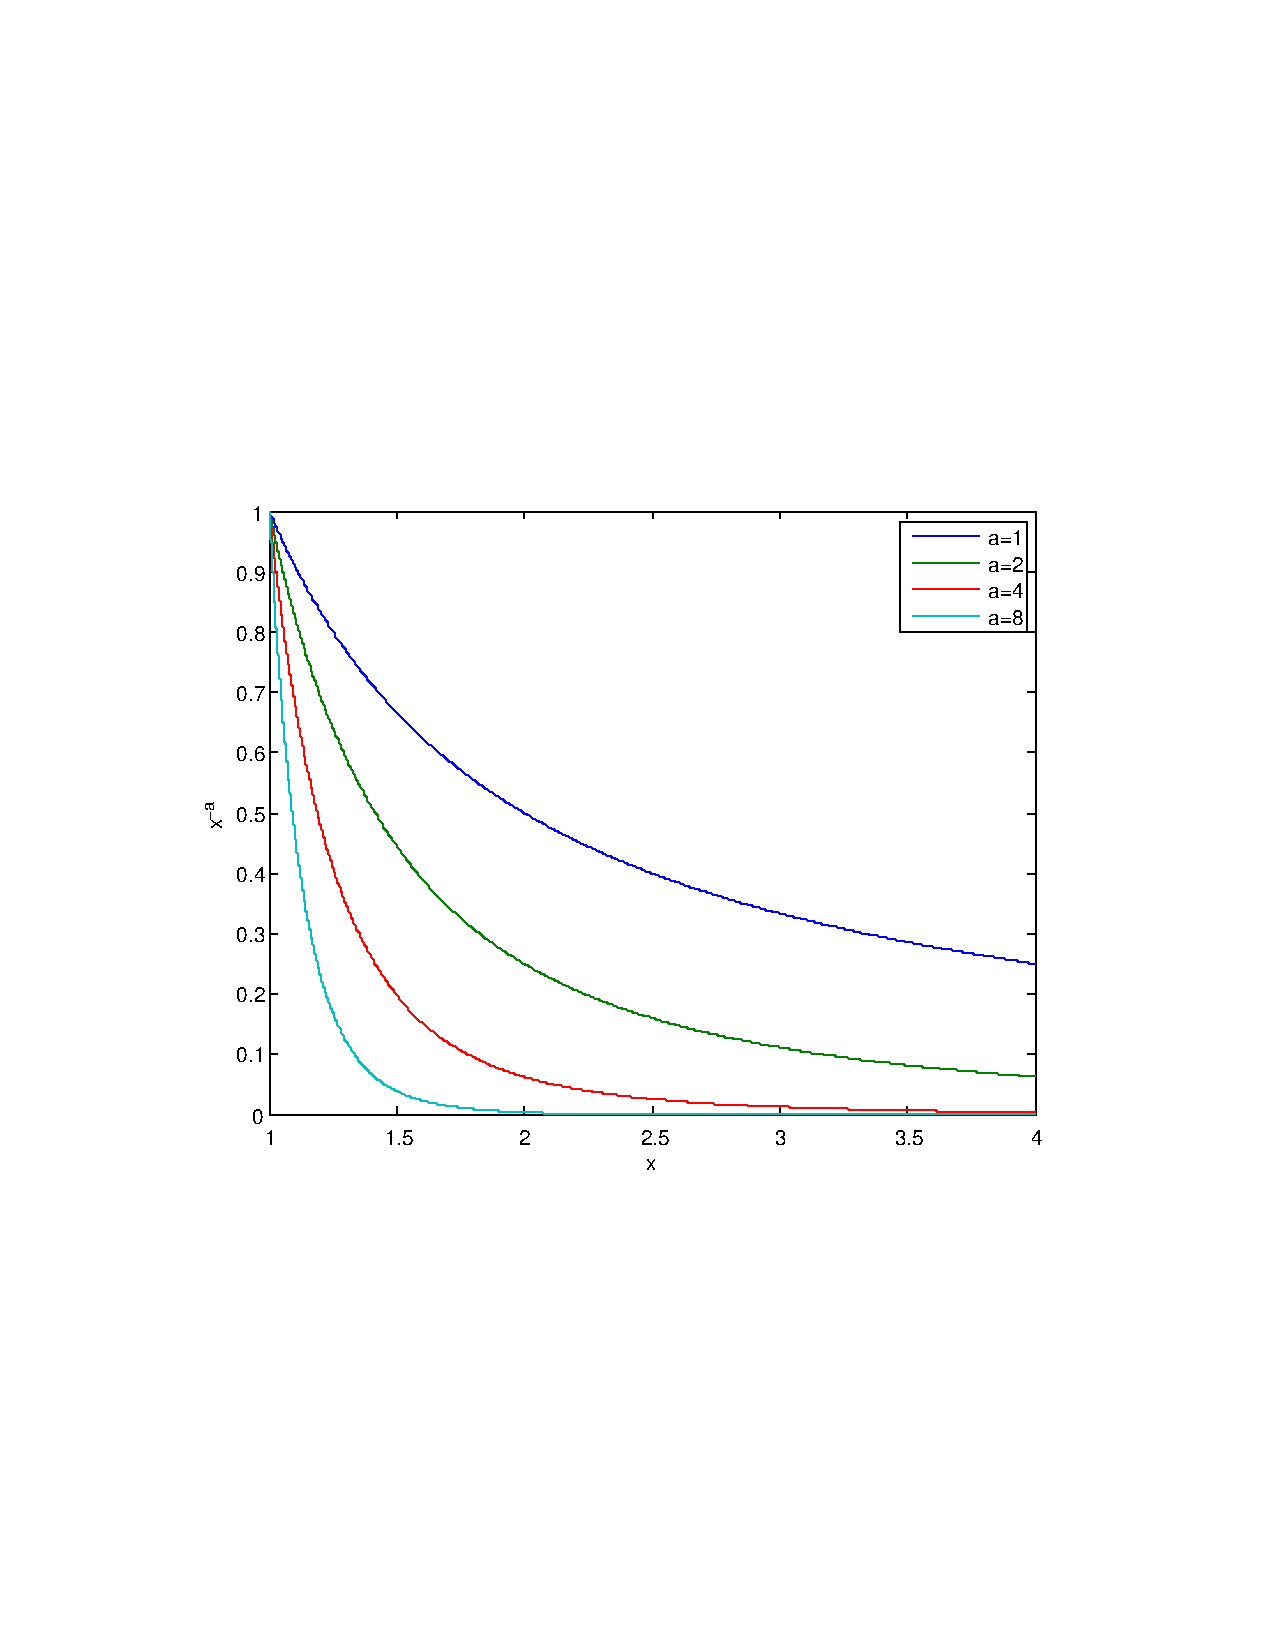
\includegraphics[width=0.4\textwidth,trim=65mm 65mm 65mm 65mm]{x-to-the-minus-a.pdf}
  \caption{$x^{-a}$ versus $x$.}
  \label{fig:x-to-the-minus-a}
\end{figure}


\section{Tracker}

The tracker uses the whisker model described in chapter 4 and
internally represents whiskers with the tuple $\coeffs$ of polynomial
coefficients.

\subsection{Filtering $\cprob{I_t}{x_t}$}

The \textsc{Importance} function in table \ref{alg:pf} is implemented
as follows. Given a hypothesis $x_t$, the tracker renders an image
$I_{x_t} = \text{Render}(x_t)$ depicting the whisker shape represented
by $x_t$. An example can be seen in figure \ref{fig:example-mask}. The
image $I_{x_t}$ is then multiplied with $I_t$. This has the result of
``masking'' the image $I_t$, extracting the pixels that the whisker
would occupy if its shape were given by $x_t$. The importance is then
calculated as the sum of the pixels of $I_{x_t} * I_t$, meaning
the importance is high if the image pixels along $x_t$ are bright.

\begin{figure}[h]
  \centering
  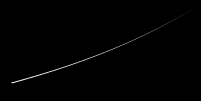
\includegraphics[width=0.38\textwidth]{example-mask.png}
  \caption{An example $I_{x_t}$.}
  \label{fig:example-mask}
\end{figure}


\section{Preprocessing of real images}

In the images of real rodents used for testing, the rodent was
illuminated from below, meaning it and its whiskers were dark against
a bright background. The filtering function described in the previous
section expects whisker pixels to be bright, so the images had to be
preprocessed.
